\chapter[A CUB-- AND LDLA--DOMAIN PROTEIN]{A CUB-- AND LDLA--DOMAIN PROTEIN ANTAGONIZES RHODOPSIN ENDOCYTOSIS TO MAINTAIN \textit{DROSOPHILA} VISUAL SENSITIVITY}                     % MUST be CAPITALIZED

This work was conducted under the direction of Dr. Hong--Sheng Li. My contribution in this work was to execute the majority of the experiments including generating transgenic flies and double mutants, western blot, immunostaining, electroretinaogram recordings and intracellular recordings, generating CULD antibody, glutathione--Sepharose binding assay and amylose resin binding assay, Arr1 binding and releasing assays. Keith Reddig and Junhai Han contributed by conducting electron microscopy. Ping Gong contributed by generating Arr1 antibody. Hong--sheng and I together wrote the abstract together and I prepared the other part of the manuscript independently.
\clearpage

%%% Abstract %%%

\section{Abstract}
The sensitivity of photoreceptor neuron to light is critical for animal vision in dim light conditions. A primary determinant of photoreceptor sensitivity is the density of the light receptor rhodopsin in photoreceptive membranes. As a G protein--coupled receptor (GPCR), the rhodopsin activity is tightly controlled by arrestins, it is surprising that visual arrestins do not significantly reduce rhodopsin concentration in the membrane during light stimulation by mediating rhodopsin endocytosis, as ??--arrestins do to non--visual GPCRs. Here we report that a CUB-- and LDLa--domain transmembrane protein CULD helps to retain \textit{Drosophila} rhodopsin in the membrane of rhabdomere, the light sensory organelle of fly photoreceptor. CULD is mostly localized in rhabdomere but is also detectable in scarce rhodopsin endocytic vesicles that contain a visual arrestin Arr1. An intracellular region of CULD interacts with Arr1 in vitro. In both \textit{culd} mutant and knockdown flies, a large fraction of rhodopsin is mislocalized in the cell body, leading to reduction of photoreceptor sensitivity. The rhodopsin internalization is due to Arr1--mediated, activity--dependent endocytosis since it was prevented by light deprivation and by mutation of endocytic factors including dynamin and Arr1. Expressing a wild--type CULD protein in photoreceptor, but not that of a mutant variant lacking the Arr1--interacting site, rescued both the rhodopsin internalization and the low sensitivity phenotypes. Once rhodopsin had been internalized in adult mutant flies, however, it was reversed only by expression of CULD, not by blocking the endocytosis. This may suggest that CULD promotes recycling of endocytic rhodopsin to the rhabdomere, probably through physically dissociating Arr1 from the endocytic rhodopsin. Given that similar CUB-- and LDLa--domain proteins are found to concentrate ionotropic neurotransmitter receptors in postsynaptic membranes of mammal and worm, CULD--like proteins may have a common role in the maintaining of receptor densities in particular membrane domains such as sensory membranes and synapses. 

\section{Introduction}
G protein--coupled receptors (GPCRs) form a large superfamily of heptahelical proteins that mediate a wide variety of biological processes, including vision, taste and smell \cite{Ferguson2001,Claing2002,Shenoy2003}. To ensure that the extracellular stimuli are translated into intracellular signals with appropriate magnitude and specificity, GPCR signaling cascade is tightly regulated. One of the major mechanisms is to modulate GPCR endocytic trafficking, which controls the amount of cell surface receptors to prevent the excitotoxicity \cite{Claing2002}. Most GPCRs undergo arrestin--mediated endocytosis. Arrestins bind to phosphorylated receptors to terminate signaling cascades and recruit APs and clathrin to induce GPCR endocytosis \cite{Claing2002,Shenoy2003,Pfleger2007}. However, GPCR endocytosis, at least temporarily, reduces the receptor level on cell surface, which reduces cell sensitivity to environmental stimuli. Limited studies have reported the mechanisms to maintain the GPCR abundance on cell surface. 

\section{Materials and Methods}
\subsection{Flies genetics and light treatment}
All examined flies except the UAS--Shits;ey--Gal4;\textit{culd} were crossed into cn,bw background to eliminate compound eye screening pigments. The genotype of wild--type flies is cn,bw. The mutant alleles used for each gene in this work are arr11, \textit{arr2}5, Gaq1, Rh1 356 and tes2. UAS--Shits was a kind gift from Dr. Scott Waddell. \textit{culd} (e01972) and Df(3L)66C--G28 were obtained from the Bloomington stock center. \textit{culd}RNAi line was obtained from VDRC stock center. Flies were reared at 21 C in dark condition or in approximate 12h light ($\sim$700lux, unless mentioned otherwise in the text)/12h dark cycles. 

\section{Results}
\subsection{Light sensitivity reduces in \textit{culd} photoreceptors}
The \textit{culd} mutant was obtained based on the microarray analysis, through which Xu et al. identified 128 eye--enriched genes \cite{Xu2004}. We examined the flies with P insertions in these genes by electroretinogram (ERG) recordings to screen for mutants with defective photoresponse. To assess the light sensitivity, fly eyes were stimulated with a series of 2s light pulses of increasing intensity (each light pulse is 5 times stronger than the previous one) and the first appearing response was recorded to calculate the relative light sensitivities \cite{Han2007}. 
 
\section{Discussion}
In this study, we have identified a \textit{Drosophila} CUB and LDLa domain protein CULD, which promotes Rh1 post--endocytic recycling, probably through dissociate Arr1 from Rh1 in endocytic vesicles. This is the first evidence to show that the light receptor rhodopsin undergoes recycling after being internalized to photoreceptor cell body. 

\begin{figure}
	\centering
		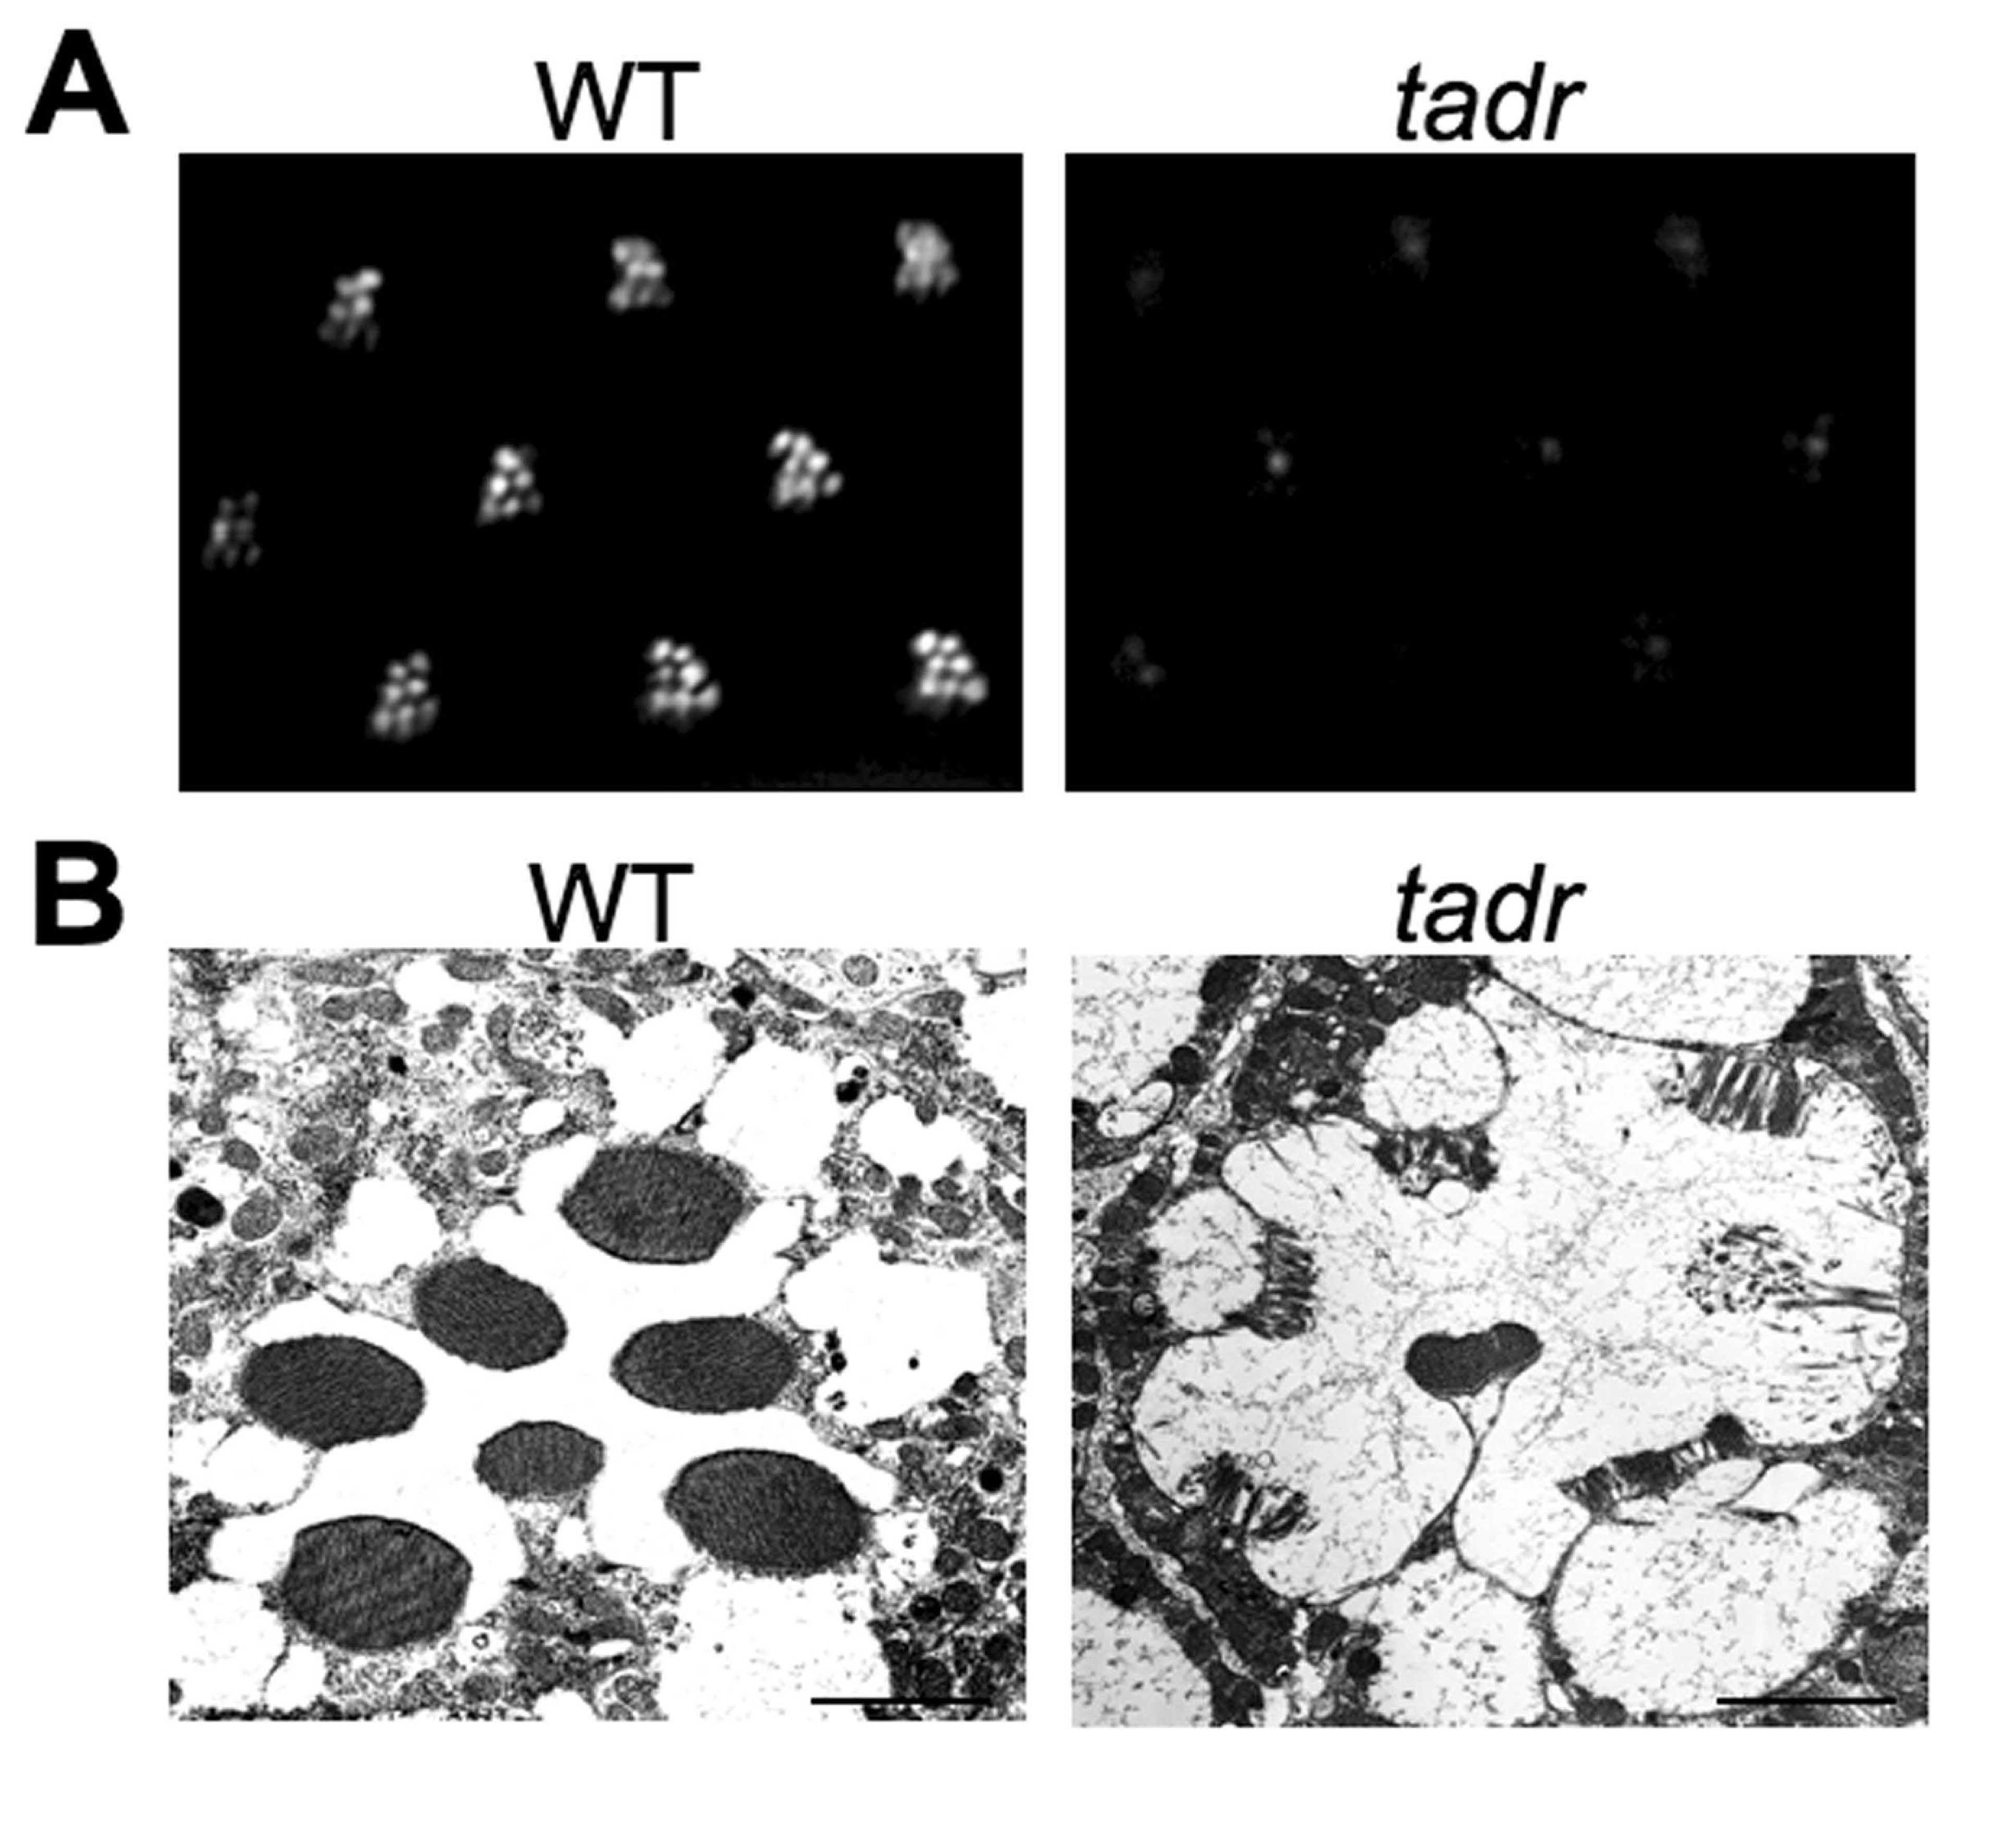
\includegraphics[width=\textwidth]{fig2-1.eps}
	\caption[short test]{leave it blank}
	\label{fig:fig3-1}
\end{figure}
\clearpage \Fref{fig:fig3-1}~long caption here.\clearpage

\begin{table}
	\caption[Short caption for the List of Table]{leave here blank}
	\centering
		\begin{tabular}{lr}
		\hline\\
			Components&Amount($\mu$L)\\
			\hline\\
			plasmid (10ng/$\mu$l) & 5\\
			forward primers(20pM) & 5\\
			reverse primers(20pM) & 5\\
			dNTP Mixture, 25mM & 10\\
			Ex taq 10X buffer & 10\\
			Takara Ex Taq(5 units/ul) & 1\\
			\hline\\
			Nuclease-Free water to a final volume of & 100\\
		\hline\\
		\end{tabular}
	\label{tab:Amplification}
\end{table}
\clearpage \Tref{tab:Oligo}--- A longer caption which is more descriptive would go here.\clearpage